\documentclass{crebsshr}

%%%%%%%%% Journal Info -- DO NOT CHANGE %%%%%%%%%
\setcounter{page}{1}
\setcounter{secnumdepth}{4}
\renewcommand\thisnumber{x}
\renewcommand\thisyear{202x}
\renewcommand\thisvolume{x}
\renewcommand\datereceived{xxxx xx, 202x}
\renewcommand\dateaccepted{xxxx xx, 202x}
\renewcommand\dateavailable{xxxx xx, 202x}
\renewcommand\doinumber{10.62366/crebss.202x.x.00x}
\renewcommand\type{XXX XXX}
\renewcommand\JEL{XXX, XXX}
%%%%%%%%% End Journal Info %%%%%%%%%

% Removed \usepackage{authblk} as it's handled by the class file
\usepackage{color}    % For text color
\usepackage{fontawesome} % For email icon
\usepackage{hyperref} % For hyperlinks
\usepackage{graphicx} % For including images

\begin{document}
    %===================================================================================================
    \markboth{Sikic}{Hrvatska u kontekstu europskih konvergencijskih klubova}
    
    \title{Hrvatska u kontekstu europskih konvergencijskih klubova}
    
    \author[L. Sikic]{Luka Sikic\thanks{Email: \href{mailto:luka.sikic@unicath.hr}{luka.sikic@unicath.hr}}}
    \address{\affilnum{1} Croatian Catholic University, Ilica 242, Zagreb, 10000, Croatia}
    
    \keywords{convergence clubs, European integration process, fractional integration, income convergence}
    
    \begin{abstract}
        Ovaj rad analizira dohodovnu konvergenciju Hrvatske u razdoblju od 2000. do 2024. godine prema četiri skupine zemalja: EU15, NMS8, NMS12 i SE4. Korištenjem metodologije vremenskih serija i frakcijske integracije, istražuje se pripadnost Hrvatske različitim konvergencijskim klubovima unutar Europske unije. Rezultati pokazuju da Hrvatska konvergira prema dohodovnim razinama EU15 i SE4, s procijenjenim parametrima frakcijske integracije od 0,87 i 0,95. To ukazuje na spor, ali postojan konvergencijski proces. Međutim, konvergencija prema NMS8 i NMS12 nije potvrđena, s parametrima iznad 1, što sugerira trajne dohodovne razlike. Ovi nalazi impliciraju da se Hrvatska ekonomski približava starim članicama EU i zemljama južne Europe, ali ne dijeli konvergencijske obrasce s novim zemljama članicama. Rezultati imaju značajne implikacije za ekonomske politike usmjerene na ubrzanje konvergencijskog procesa.
    \end{abstract}

    \maketitle
    \bigskip
    \noindent

    %--------------------------------------------------------------------------------------------------- 
    \section{Uvod}

    Dohodovna konvergencija predstavlja ključni aspekt ekonomske integracije i razvoja, posebno unutar Europske unije koja teži smanjenju ekonomskih dispariteta među svojim članicama. Za Hrvatsku, kao najnoviju članicu EU, razumijevanje dinamike dohodovne konvergencije je od posebne važnosti. Ovo istraživanje ima za cilj analizirati pripadnost Hrvatske različitim konvergencijskim klubovima unutar EU te utvrditi u kojoj mjeri Hrvatska smanjuje dohodovni jaz s drugim zemljama članicama. U radu istražuje se dohodovna konvergencija Hrvatske prema različitim skupinama europskih zemalja: stare članice EU (EU15), nove članice iz srednje i istočne Europe (NMS8 i NMS12) te zemlje južne Europe (SE4). Korištenjem metoda vremenskih serija i frakcijske integracije, istraživanje pruža uvid u konvergencijske procese koji oblikuju ekonomski položaj Hrvatske unutar EU.
    
    Rad doprinosi postojećoj literaturi na području ekonomske konvergencije kroz nekoliko ključnih aspekata. Prvo, fokusiranje na Hrvatsku u razdoblju od 2000. do 2024. godine pruža ažurirani uvid u dinamičke ekonomske promjene tijekom dugog vremenskog razdoblja, koje uključuje i proširivanja Europske unije. Drugo, primjena metodologije vremenskih serija i frakcijske integracije \citep{Silverberg1999, Cuñado2006, Mello2007, Ayala2012} omogućava dublje razumijevanje dugoročnih trendova i privremenih fluktuacija u dohodovnim razlikama, čime se nadilaze tradicionalne metode. Ovaj pristup također pruža preciznije procjene parametara konvergencije, što doprinosi sofisticiranijem razumijevanju konvergencijskih procesa. Treće, istraživanje pripadnosti Hrvatske različitim konvergencijskim klubovima unutar Europske unije doprinosi diferenciranom pristupu u analizi ekonomskih integracija. Četvrto, rezultati ovog rada imaju praktične implikacije za ekonomske politike Hrvatske.
    
    U nastavku rada pruža se pregled ključnih aspekata literature o dohodovnoj konvergenciji te pregled radova koji su analizirali konvergenciju dohotka u europskim posttranzicijskim zemljama. U trećem dijelu opisuju se koncepti dohodovne konvergencije u okviru analize vremenskih serija te se detaljno prikazuje metodologija frakcijske integracije i korišteni procjenitelji. Četvrti dio donosi stilizirane činjenice o konvergencijskom procesu Republike Hrvatske prema dohodovnim razinama skupina EU15, NMS8, NMS12 i SE4, dok su u petom dijelu prikazani rezultati istraživanja. U zaključku se sumiraju glavne spoznaje analize.
    
    \section{Pregled literature o dohodovnoj konvergenciji}
    
    Rana literatura o konvergenciji prvenstveno se usmjeravala na provjeru ekonomske teorije rasta \citep{Barro1990, Barro1991, Mankiw1992} koristeći uglavnom prostornu (eng. cross-section) regresijsku analizu. Neki autori primijenili su različite procjenitelje za panel-podatke \citep{Knight1993, Islam1995, Caselli1996, Lee1998, Bond2001}. Općenito, rezultati su potvrdili postojanje apsolutne ili uvjetne konvergencije u globalnim uzorcima zemalja, pri čemu su procijenjene stope konvergencije iznosile između 2\% i 4\%. Ipak, nije uspostavljen jedinstven konsenzus o globalnoj dohodovnoj konvergenciji.
    
    U kasnijoj fazi, naglasak se pomaknuo na primjenu različitih metoda testiranja dohodovne konvergencije. Bernard i Durlauf \citeyearpar{Bernard1991} prvi su analizirali dohodovnu konvergenciju u okviru metodologije vremenskih serija. U kasnijim radovima \citep{Bernard1995, Bernard1996} istaknuli su da tehnike vremenskih serija imaju poželjnija empirijska svojstva u odnosu na prostornu analizu. Oni uvode pojam stohastičke konvergencije, koji se odnosi na testiranje jediničnog korijena u razlikama BDP-a po stanovniku između dviju zemalja.
    
    Bernard i Durlauf \citeyearpar{Bernard1995} testirali su stohastičku konvergenciju primjenom testova jediničnog korijena na razlikama dohotka 15 zemalja OECD-a u odnosu na grupni prosjek. Nisu pronašli uvjerljive dokaze za dugoročnu konvergenciju u svim državama, no potvrdili su konvergenciju za manju skupinu europskih zemalja. Jones \citeyearpar{Jones2002} je, koristeći metodologiju jediničnog korijena i koncept stohastičke konvergencije, analizirao zapadnoafričke države te zaključio da ne postoje značajni dokazi za konvergenciju u cjelokupnom uzorku. Pesaran \citeyearpar{Pesaran2007} primijenio je ADF i KPSS testove stacionarnosti razlika dohotka između parova zemalja za uzorke od 56, 99 i 101 države tijekom različitih razdoblja od 1950. do 2000. godine. U oko 72\% slučajeva potvrdio je konvergencijsku hipotezu, ukazujući tako na formiranje ``klubova konvergencije'' – skupina zemalja koje konvergiraju, ali ne na univerzalnoj razini.
    
    Istraživanja dohodovne konvergencije temeljena na analizi vremenskih serija kasnije su proširena na panel-podatke, uključujući testove stacionarnosti i kointegracijske analize. Evans i Karras \citeyearpar{Evans1996a} potvrdili su konvergenciju između 48 američkih saveznih država i 54 zemlje koristeći test jediničnog korijena za panel-podatke \citep{LevinLin1993}. U drugom radu, Evans i Karras \citeyearpar{Evans1996b} istražili su apsolutnu konvergenciju između saveznih država SAD-a, no nisu pronašli empirijsku potvrdu za taj oblik konvergencije. Fleissig i Strauss \citeyearpar{Fleissig2001} primijenili su testove jediničnog korijena za analizu dugoročne konvergencije u 15 OECD zemalja i europskih zemalja u razdoblju od 1900. do 1987. te zaključili da je konvergencija potvrđena nakon Drugog svjetskog rata, ali ne i za cjelokupni period. Kim \citeyearpar{Kim2005} je, koristeći panel-kointegracijski test na uzorku od 13 korejskih regija, također potvrdio konvergenciju, dok su Carrion-i-Silvestre i suradnici \citeyearpar{Carrion2005} pomoću panel-testova jediničnog korijena zaključili da postoji konvergencija između 13 azijskih zemalja.
    
    Relativno mali broj radova o dohodovnoj konvergenciji primijenio je metodologiju frakcijske integracije. Ti su radovi upozorili na ograničenja testova jediničnog korijena i kointegracije, uglavnom zbog njihove statističke osjetljivosti te činjenice da se kointegracijski parametar obično ograničava samo na vrijednosti 0 ili 1. Budući da je konvergencija proces dugog trajanja, frakcijska integracija naglašava potrebu za variranjem integracijskog parametra u rasponu od 0 do 1 radi obuhvaćanja procesa ``duge memorije''. Michelacci i Zaffaroni \citeyearpar{Michelacci2000} predlažu primjenu standardnih testova stacionarnosti kao početni korak u analizi dohodovnih serija, pokazujući da je u frakcijskom kontekstu konvergencijska stopa od 2\% odgovarajuća za integracijski parametar između 0,5 i 1. Time su potvrdili rezultate dobivene prostornom regresijskom analizom te zaključili da je ovaj pristup kompatibilan s metodama vremenskih serija.
    
    U primjeni frakcijske integracije na empirijske primjere, Cuñado i suradnici \citeyearpar{Cuñado2003} ispitali su konvergenciju Australije, Japana, Kanade i Ujedinjenog Kraljevstva prema dohodovnom prosjeku SAD-a. Rezultati su potvrdili konvergenciju za Australiju i Kanadu, dok su za Ujedinjeno Kraljevstvo dokazi bili manje uvjerljivi, a konvergencija za Japan nije mogla biti potvrđena. Ayala i suradnici \citeyearpar{Ayala2012} primijenili su frakcijsku integraciju na uzorak od 17 zemalja Latinske Amerike u odnosu na SAD za razdoblje od 1950. do 2008. godine i nisu pronašli dokaze stohastičke konvergencije ni za jednu promatranu zemlju. Kamal i Arteche \citeyearpar{Kamal2014} također su primijenili frakcijsku integraciju i nisu potvrdili dohodovnu konvergenciju među španjolskim regijama. Ovi rezultati ističu važnost frakcijske integracije u analizi dugoročnih kretanja, zahvaljujući njezinoj sposobnosti obuhvaćanja procesa duge memorije te većoj fleksibilnosti u odnosu na tradicionalne testove jediničnog korijena i kointegracije. Takav pristup omogućuje dublje razumijevanje dinamike konvergencije i pomaže u prepoznavanju specifičnih obrazaca unutar različitih skupina zemalja.
    
    \subsection{Dohodovna konvergencija u EU posttranzicijskim zemljama}
    
    Istraživanja o dohodovnoj konvergenciji u europskim posttranzicijskim zemljama obuhvatila su raznolike skupine zemalja, različite aspekte ekonomske konvergencije te su koristila širok spektar metodoloških pristupa. Jedna skupina istraživanja fokusirala se na beta i sigma konvergenciju u novim zemljama članicama EU, primjenjujući prostorne i panel analize, dok su drugi radovi koristili metodologiju vremenskih serija. Različite duljine analiziranih vremenskih razdoblja među istraživanjima otežavale su usporedivost rezultata. Druga skupina istraživanja proučavala je konvergenciju makroekonomskih indikatora u posttranzicijskim zemljama prema europskim standardima.
    
    Kočenda \citeyearpar{Kočenda2001} analizirao je konvergenciju makroekonomskih indikatora za zemlje Srednje i Istočne Europe prema europskom prosjeku u razdoblju od 1991. do 1998. godine. Rezultati su pokazali konvergenciju u većini zemalja i indikatora, s najizraženijom konvergencijom u dohotku te bržim napretkom baltičkih zemalja. Dobrinsky \citeyearpar{Dobrinsky2003} fokusirao se na dohodovnu konvergenciju novih članica EU, ukazujući da se pozitivan trend konvergencije prema europskim razinama pojavio nakon sredine 1990-ih godina. Kutan i Yigit \citeyearpar{Kutan2004} istraživali su nominalnu i realnu konvergenciju u pet skupina europskih tranzicijskih zemalja u razdoblju od 1993. do 2000. godine, potvrđujući niži stupanj nominalne i realne konvergencije. Vojinović i Oplotnik \citeyearpar{Vojinović2004} analizirali su uvjetnu beta i sigma konvergenciju zemalja koje su pristupile EU 2004. godine, otkrivajući ubrzanu konvergenciju u razdoblju od 1995. do 2006. godine. Kočenda i suradnici \citeyearpar{Kočenda2006} ispitali su nominalnu i realnu konvergenciju deset novih članica EU, pri čemu su utvrdili sporu dohodovnu konvergenciju, ali bržu nominalnu konvergenciju.
    
    Brüggemann i Trenkler \citeyearpar{Brueggemann2007} primijenili su testove jediničnog korijena za analizu dohodovne konvergencije Češke, Poljske i Mađarske prema EU15 i mediteranskim zemljama, potvrđujući konvergenciju za Češku i Mađarsku. Rapacki i Próchniak \citeyearpar{Rapacki2009} istraživali su apsolutnu i uvjetnu beta konvergenciju te sigma konvergenciju u 27 bivših socijalističkih zemalja od 1990. do 2005. godine, zaključujući da Srednja i Istočna Europa imaju različite konvergencijske obrasce u usporedbi sa zemljama Zajednice nezavisnih država (CIS). Ignazzi i Zdárek \citeyearpar{Ignazzi2009} analizirali su dohodovnu konvergenciju novih članica EU koristeći različite metodologije, te su zaključili da konvergencija postoji, ali nije postojana. Vojinović, Acharya i Próchniak \citeyearpar{Vojinović2009} potvrdili su beta i sigma konvergenciju za deset zemalja koje su postale članice EU 2004. godine, s ubrzanom konvergencijom od sredine 1990-ih do 2000-ih, potaknutoj integracijom s EU.
    
    Nekoliko istraživanja potvrdilo je dohodovnu konvergenciju posttranzicijskih zemalja prema europskom centru \citep{Monfort2013, Próchniak2013, Szeles2010} u razdoblju do posljednjeg proširenja Europske unije. Dokazi također ukazuju na nastavak konvergencijskog procesa i nakon globalne financijske krize \citep{Åslund2018}. Međutim, literatura općenito nije postigla konsenzus o tome hoće li proces konvergencije posttranzicijskih zemalja biti dovršen \citep{Papi2018}. Unatoč tome, dokazi sugeriraju da je članstvo u Europskoj uniji bilo ključno za nastavak približavanja tih zemalja europskom dohotovnom prosjeku \citep{Rapacki2019}.
    
    Navedena istraživanja ističu kompleksnost procesa dohodovne konvergencije u posttranzicijskim zemljama te ukazuju na važnost kontinuiranog praćenja i analize kako bi se bolje razumjeli čimbenici koji utječu na uspješnost konvergencije. Različiti metodološki pristupi i vremenski horizonti istraživanja naglašavaju potrebu za standardizacijom metodologije kako bi se omogućila veća usporedivost rezultata i donošenje informiranijih zaključaka o konvergencijskim trendovima unutar Europske unije. Ovaj rad popunjava tu prazninu pružajući ažuriranu i detaljnu analizu dohodovne konvergencije Hrvatske, koristeći metode frakcijske integracije.

\section{Metodologija}
    
    \subsection{Koncepti dohodovne konvergencije u okviru metodologije vremenskih serija i frakcijska integracija}
    
    U metodologiji vremenskih serija poznata su dva temeljna konvergencijska koncepta: apsolutna i uvjetna konvergencija. Dohodovna konvergencija može se definirati kao:
    
    \begin{equation} \label{eq:eq1}
    \lim_{k \to \infty} E(y_{i,t+k} - y_{j,t+k} \mid I_t) = 0
    \end{equation}
    
    gdje je dohodak u danom periodu definiran kao \( y_t = \ln(Y_t) \), \( y_{i,t} \) označava dohodak u zemlji \( i \) u trenutku \( t \), \( y_{j,t} \) je dohodak u zemlji \( j \) u istom razdoblju, dok \( I_t \) označava set raspoloživih informacija u danom periodu. Jednadžba (\ref{eq:eq1}) označava da je razlika dohotka zemlje \( i \) i \( j \) stacionaran proces sa prosjekom nula. Ovaj koncept, poznat kao deterministička konvergencija, povezuje se s Bernardom i Durlaufom (1995) \citep{Bernard1995}.
    
    Proširenjem definicije (\ref{eq:eq1}):
    
    \begin{equation} \label{eq:eq2}
    \lim_{k \to \infty} E(y_{i,t+k} - y_{j,t+k} \mid I_t) = \beta
    \end{equation}
    
    gdje \( \beta \) označava konstantu, (\ref{eq:eq1}) predstavlja definiciju apsolutne konvergencije, dok se (\ref{eq:eq2}) odnosi na uvjetnu konvergenciju. Jednadžba (\ref{eq:eq2}) označava da će dvije zemlje konvergirati uz postojanje konstantnog dohodovnog jaza jednakog \( \beta \). Ovaj koncept stohastičke konvergencije, povezan s Carlinom i Millsom (1993) \citep{Carlin1993}, implicira da je razlika dohotka zemalja \( i \) i \( j \) trend stacionaran proces.
    
    Pošto se konvergencijski koncepti (\ref{eq:eq1}) i (\ref{eq:eq2}) odnose na logaritmirane vrijednosti, izražene kao:
    
    \begin{equation} \label{eq:eq3}
    \log\left(\frac{y_{i,t}}{y_{j,t}}\right)
    \end{equation}
    
    Apsolutna konvergencija prema definiciji (\ref{eq:eq3}) izražava se kao:
    
    \begin{equation} \label{eq:eq4}
    \log\left(\frac{y_{i,t}}{y_{j,t}}\right) = \alpha + \epsilon_{i,j,t}
    \end{equation}
    
    Uvjetna konvergencija definirana je kao:
    
    \begin{equation} \label{eq:eq5}
    \log\left(\frac{y_{i,t}}{y_{j,t}}\right) = \beta + \alpha + \epsilon_{i,j,t}
    \end{equation}
    
    Statistička analiza dohodovne konvergencije može se provesti testom jediničnog korijena u vremenskoj seriji razlike dohotka zemalja \( i \) i \( j \), kako predlažu Carlino i Mills (1993) \citep{Carlin1993}. Druga metoda je kointegracijska analiza, predložena od strane Bernarda i Durlaufa (1995) \citep{Bernard1995}. Da bi se ekonomski koncepti dohodovne konvergencije ekonometrijski testirali, definiramo:
    
    \begin{equation} \label{eq:eq6}
    y_{i,j,t} = \log\left(\frac{Y_{i,t}}{Y_{j,t}}\right)
    \end{equation}
    
    gdje \( y_{i,j,t} \) predstavlja razliku logaritama dohotka u zemlji \( i \) i \( j \). Uz definicije dohodovne konvergencije (\ref{eq:eq1}) i (\ref{eq:eq2}) te uzimajući u obzir da \( I_t \) označava informacijski set u trenutku \( t \), jednadžba (\ref{eq:eq6}) se može kompaktno zapisati:
    
    \begin{equation} \label{eq:eq7}
    y_{i,j,t} = \alpha + \epsilon_{i,j,t}
    \end{equation}
    
    Model (\ref{eq:eq6}) može se asimptotski izraziti kao:
    
    \begin{equation} \label{eq:eq8}
    y_{i,j,t} = \beta + \alpha + \epsilon_{i,j,t}
    \end{equation}
    
    iz čega slijedi da svaka situacija gdje \( \beta = 0 \) implicira konvergenciju uz konstantnu dohodovnu razliku. Ovo postaje jasnije preuređenjem jednadžbe (\ref{eq:eq8}):
    
    \begin{equation} \label{eq:eq9}
    \Delta y_{i,j,t} = \epsilon_{i,j,t}
    \end{equation}
    
    \subsection{Frakcijska integracija}
    
    Koncept frakcijske integracije je uveden u makroekonometrijsku literaturu radovima Granger (1980, 1981), Granger i Joyeux (1980), te Hosking (1981) \citep{Granger1980, Granger1981, GrangerJoyeux1980, Hosking1981}. Ovim konceptom se nastojalo opisati snažno autokorelirane procese za koje je karakteristična povezanost među međusobno udaljenim realizacijama.
    
    Ukoliko je neka vremenska serija integrirana reda \( z=0 \), može se reći kako je riječ o procesu kratke memorije čija autokorelacijska funkcija brzo opada, dok integracijski parametar \( z=1 \) označava nestacionarnost i perzistentnost šokova u takvoj vremenskoj seriji. Od statističkog i ekonomskog interesa je analizirati da li integracijski parametar poprima neku necjelobrojnu vrijednost unutar intervala \( 0<z<1 \).
    
    Primjerice, ukoliko \( 0<z<0.5 \), vremenska serija je stacionarna, no njena autokorelacijska funkcija će opadati sporije nego u slučaju \( z=0 \). Slučaj kada parametar integracije leži u intervalu \( 0.5<z<1 \) označava vremensku seriju koja je nestacionarna, no reverzibilna prema prosjeku. Tada je riječ o procesu duge memorije koji nije kovarijančno stacionaran, no šokovi će ipak nestati iz serije u dugom roku.
    
    \subsection{Frakcijski integrirani proces}
    
    Nadovezujući se na prethodne radove, frakcijski integrirani proces dohodovnih razlika između zemlje \( i \) i \( j \) se može zapisati u obliku:
    
    \begin{equation} \label{eq:eq10}
    (1-L)^z (y_{i,t} - y_{j,t}) = \epsilon_t
    \end{equation}
    
    gdje je \( L \) operator pomaka i definiran je kao \( L^k y_t = y_{t-k} \), \( \epsilon_t \) označava standardnu pogrešku modela za koju se pretpostavlja da je opisana stohastičkim procesom bijelog šuma koji ima prosjek nula i konstantnu varijancu.
    
    Jednadžbu (\ref{eq:eq10}) je sada moguće izraziti u generalnijem obliku pogodnom za empirijsko testiranje:
    
    \begin{equation} \label{eq:eq11}
    \phi(L)(1-L)^z (y_{i,t} - y_{j,t}) = \theta(L)\epsilon_t
    \end{equation}
    
    gdje je \( \phi(L) \) autoregresivni polinom pomaka definiran kao \( \phi(L) = 1 - \phi_1 L - \phi_2 L^2 - \dots - \phi_p L^p \), \( \theta(L) \) je polinom pomičnog prosjeka operatora pomaka i opisan je kao \( \theta(L) = 1 + \theta_1 L + \theta_2 L^2 + \dots + \theta_q L^q \), dok \( (1-L)^z \) predstavlja operator frakcijske diferencije u obliku:
    
    \begin{equation} \label{eq:eq12}
    (1-L)^z = \sum_{k=0}^{\infty} \frac{\Gamma(k-z)}{\Gamma(-z)\Gamma(k+1)} L^k
    \end{equation}
    
    Pri tome \( \Gamma(\cdot) \) označava generaliziranu faktorsku gama funkciju.
    
    Invertiranje jednadžbe (\ref{eq:eq11}) je moguće u slučaju kada parametar \( z \) frakcijske integracije leži u intervalu \( 0<z<0.5 \), te je tada moguće je zapisati:
    
    \begin{equation} \label{eq:eq13}
    y_{i,t} - y_{j,t} = \frac{\theta(L)}{\phi(L)}(1-L)^{-z}\epsilon_t
    \end{equation}
    
    iz čega je vidljivo da \( \phi(L) \) opisuje kratkoročnu dinamiku procesa, dok su njegovi dugoročni efekti obuhvaćeni izrazom za frakcijsku integraciju \( (1-L)^{-z} \).
    
    U slučaju kada je \( z \) invertibilnost u (\ref{eq:eq13}) moguća, proces (\ref{eq:eq11}) je stacionaran. U kontekstu ovog rada je od posebnog interesa slučaj u kojem parametar frakcijske integracije leži u intervalu \( 0.5<z<1 \). Tada je riječ o nestacionarnom procesu koji ima tendenciju vraćanja prema prosjeku (mean-reverting).
    
    Za proces koji ima tendenciju vraćanja prema prosječnoj vrijednosti je karakteristično da funkcija kumulativnih impulsnih šokova asimptotski teži nuli. Upravo se tu očituje dodatna fleksibilnost pristupa frakcijske kointegracije u odnosu na pristup testiranja stacionarnosti ili kointegracije.
    
    Naime, parametar frakcijske integracije koji iznosi manje od jediničnog označava kako će šok vremenske serije \( \epsilon_t \) odumrijeti čak i u slučaju da je ta vremenska serija ima karakteristike nestacionarnog procesa. Mello i Guimarães-Filho \citeyearpar{Mello2007} dokazuju kako je u tom slučaju koncept uvjetne dohodovne konvergencije dobro opisan frakcijski integriranim procesom (\ref{eq:eq11}).
    
    \subsection{Empirijska Specifikacija}
    
    Empirijska specifikacija konvergencije se u ovom radu odnosi na dohodovni diferencijal između Hrvatske i dohodovnog prosjeka četiri grupe zemalja EU15, NMS8, NMS12 te SE4. Budući da se prosjek grupe zemalja koristi kao konvergencijski benchmark, model (\ref{eq:eq6}) je potrebno preinačiti na način:
    
    \begin{equation} \label{eq:eq14}
    \phi(L)(1-L)^z (\log y_{HR,t} - \log y_{avg,t}) = \theta(L)\epsilon_t
    \end{equation}
    
    gdje \( \log y_{avg,t} \) označava dohodovni prosjek \( j \) zemalja svake od četiri navedene grupe i definiran je kao:
    
    \begin{equation} \label{eq:eq15}
    \log y_{avg,t} = \frac{1}{n}\sum_{j=1}^{n} \log y_{j,t}
    \end{equation}
    
    To implicira konačnu empirijsku specifikaciju dohodovnog diferencijala u obliku:
    
    \begin{equation} \label{eq:eq16}
    y_{HR,t} - y_{avg,t} = \frac{\theta(L)}{\phi(L)}(1-L)^{-z}\epsilon_t
    \end{equation}

\section{Korišteni podaci i stilizirane činjenice o konvergencijskom procesu Hrvatske}

U istraživanju se koriste vremenske serije BDP-a Hrvatske i nekoliko skupina zemalja u razdoblju od početka 2000. do kraja 2023. godine: stare zemlje članice Europske Unije (EU15), nove zemlje članice (NMS8 i NMS12) te zemlje juga Europe (SE4). Pri tome se koriste EUROSTAT-ovi podatci BDP-a na kvartalnoj frekvenciji u razdoblju od 2000q1 do 2023q4. EUROSTAT baza objavljuje podatke za kvartalni BDP bez korekcije za broj stanovnika pa je zbog toga dodatno korištena IMF-ova baza World Economic Outlook iz koje su preuzeti godišnji podatci o stanovništvu u periodu od 2000. godine do 2023. godine za sve zemlje obuhvaćene analizom. Godišnji podatci za stanovništvo su metodom kubične interpolacije svedeni na kvartalne, nakon čega su korišteni u formiranju vremenske serije BDP per capita na kvartalnoj frekvenciji.

\begin{figure}[ht]
\centering
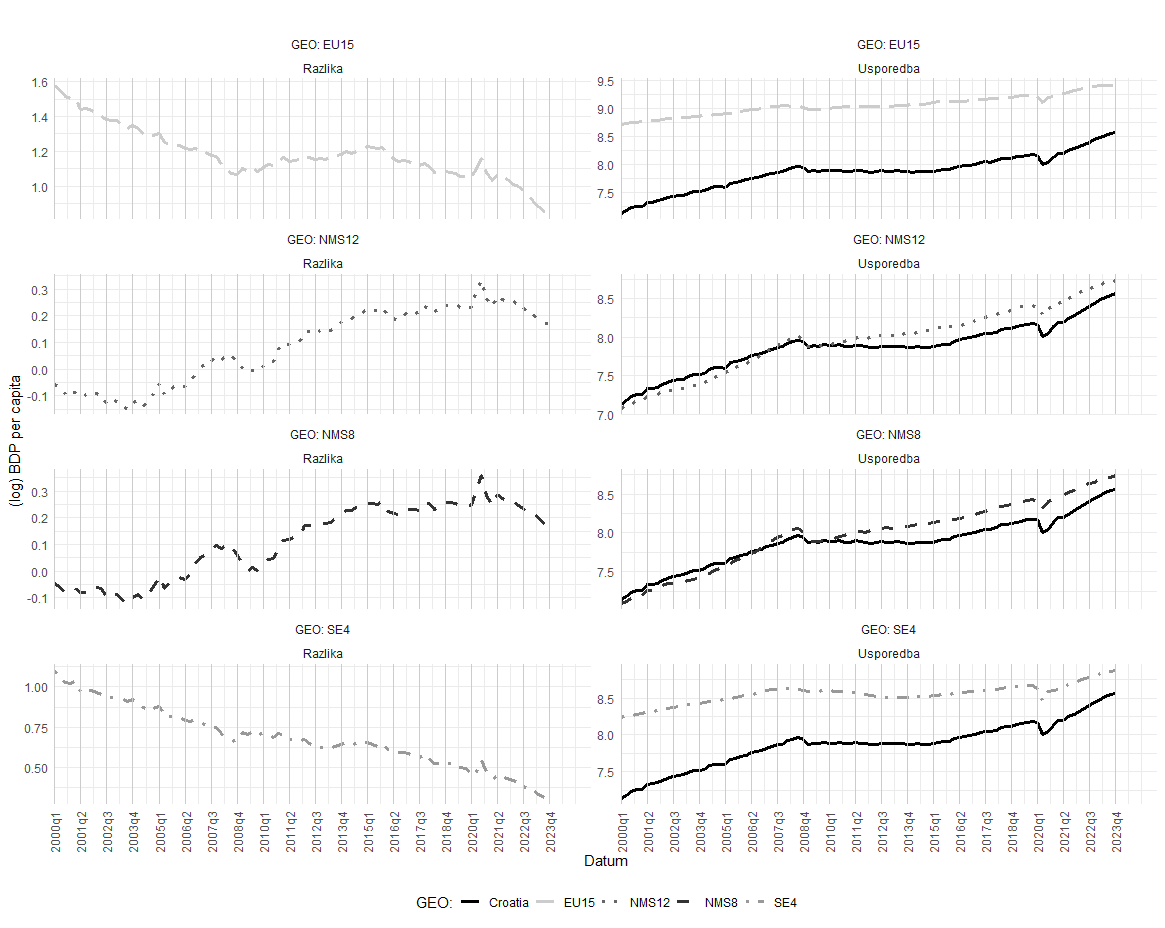
\includegraphics[width=\linewidth]{Rplot.png} % Zamijenite 'Rplot.png' sa stvarnom putanjom vaše slike
\caption{Kretanje razlika u BDP-u po stanovniku između Hrvatske i analiziranih skupina zemalja.}
\label{fig:grafikon1}
\end{figure}

Slika \ref{fig:grafikon1} pruža vizualni prikaz kretanja razlika u BDP-u po stanovniku između Hrvatske i analiziranih skupina zemalja. U gornjem panelu prikazano je kretanje BDP-a po stanovniku za Hrvatsku i EU15. Do globalne ekonomske krize 2007. godine, Hrvatska je bilježila brži rast BDP-a, značajno se približavajući prosjeku EU15. Međutim, nakon izbijanja krize dolazi do korekcije hrvatskog BDP-a. Dok se EU15 postupno oporavlja i nastavlja s rastom, hrvatski dohodak stagnira ili čak opada. U novijem razdoblju, nakon krize uzrokovane pandemijom COVID-19, hrvatski BDP ponovno ubrzava rast, pokazujući obnovljeni trend približavanja prosjeku EU15.

Središnja dva panela prikazuju usporedbu Hrvatske s NMS8 i NMS12. Zanimljivo je da su do 2007. godine sve zemlje imale podjednake stope rasta, sugerirajući zajedničku konvergenciju. No, nakon krize, hrvatsko gospodarstvo počinje usporavati ili stagnirati, dok NMS8 i NMS12 bilježe nastavak snažnijeg rasta. To je rezultiralo rastućim jazom između BDP Hrvatske i tih dviju skupina. Ipak, u novije vrijeme, osobito nakon COVID-19 krize, primjetan je novi zamah u hrvatskom gospodarstvu, što dovodi do ublažavanja dohodovnog jaza u odnosu na NMS8 i NMS12. Zadnji panel pruža pregled odnosa Hrvatske prema SE4 skupini. Tijekom cijelog promatranog razdoblja vidljiva je stabilnija konvergencija: unatoč kratkotrajnom usporavanju tijekom krize 2007. godine, Hrvatska je kontinuirano bilježila brži rast od SE4, potvrđujući dugoročnu tendenciju konvergiranja prema toj skupini.

Iz prikazanih podataka može se zaključiti kako Hrvatska u dugom roku nastavlja konvergirati prema prosjeku EU15 i SE4. Iako je konvergencija prema NMS8 i NMS12 neko vrijeme bila zaustavljena ili usporena, osobito od 2007. do razdoblja nakon COVID-19 krize, najnoviji podatci upućuju na to da je i prema tim skupinama ponovno započeo proces približavanja. Kriza iz 2007. godine zaustavila je konvergenciju prema EU15 samo privremeno, dok je kretanje prema SE4 ostalo postojano. U novijem, postpandemijskom razdoblju, Hrvatska pokazuje pojačanu gospodarsku vitalnost, podržavajući daljnje smanjenje dohodovnih razlika u odnosu na sve analizirane skupine zemalja.

%==========================================================================================================================================
\section{Rezultati analize}

Nakon deskriptivne analize podataka, u ovom dijelu predstavljeni su rezultati statističkih testova dohodovne konvergencije između Hrvatske i skupina EU15, NMS8, NMS12 te SE4. Rezultati su dobiveni korištenjem proširenog Dickey-Fuller (ADF) testa te dvaju procjenitelja frakcijske integracije, konkretno procjenitelja koje su predložili Geweke i Porter-Hudak (1983) \citep{Geweke1983} te Reisen (1994) \citep{Reisen1994}. Prije provođenja ovih statističkih testova, provedeni su Ljung-Box test i analiza autokorelacijske funkcije (ACF) za 20 vremenskih zaostataka kako bi se procijenila prikladnost korištene metodologije.

\begin{table}[ht]
\centering
\caption{Ljung-Box Test, P-val}
\label{tab:tablica1}
\begin{tabular}{lcccccccccc}
\toprule
\textbf{Group} & \textbf{Lag 2} & \textbf{Lag 4} & \textbf{Lag 6} & \textbf{Lag 8} & \textbf{Lag 10} & \textbf{Lag 12} & \textbf{Lag 14} & \textbf{Lag 16} & \textbf{Lag 18} & \textbf{Lag 20} \\
\midrule
EU15  & 0 & 0 & 0 & 0 & 0 & 0 & 0 & 0 & 0 & 0 \\
NMS12 & 0 & 0 & 0 & 0 & 0 & 0 & 0 & 0 & 0 & 0 \\
NMS8  & 0 & 0 & 0 & 0 & 0 & 0 & 0 & 0 & 0 & 0 \\
SE4   & 0 & 0 & 0 & 0 & 0 & 0 & 0 & 0 & 0 & 0 \\
\bottomrule
\end{tabular}
\end{table}

Tablica \ref{tab:tablica1} prikazuje p-vrijednosti od 0 za sve vremenske zaostatke u Ljung-Box testu, što ukazuje na odbacivanje nulte hipoteze o nepostojanju autokorelacije. Ovaj rezultat sugerira značajnu autokorelaciju kroz sve vremenske zaostatke, implicirajući da prošle vrijednosti imaju snažan i statistički značajan utjecaj na buduće vrijednosti tijekom cijelog promatranog razdoblja. Prisustvo autokorelacije na višestrukim zaostacima ukazuje da podatke karakterizira dugo pamćenje ili perzistentnost, što znači da se utjecaj prošlih šokova sporo smanjuje tijekom vremena, a povijesne vrijednosti serije nastavljaju utjecati na buduća opažanja kroz dulje vremensko razdoblje.

S obzirom na ovako izraženu strukturu autokorelacije, konvencionalni modeli vremenskih serija koji pretpostavljaju procese kratkog pamćenja neće adekvatno uvažiti temeljnu dinamiku podataka. Stoga je nužno primijeniti modele koji mogu uzeti u obzir dugoročne ovisnosti, poput procjenitelja frakcijske integracije, koji su prikladni za modeliranje i predviđanje u prisutnosti karakteristika dugog pamćenja.

\begin{figure}[ht]
\centering
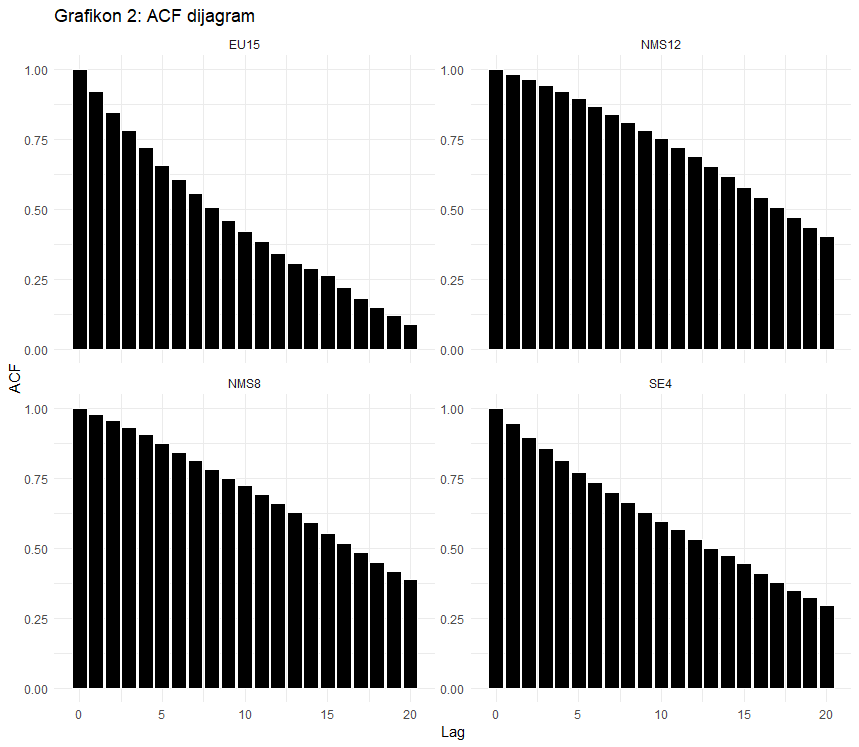
\includegraphics[width=\linewidth]{Rplot01.png} % Zamijenite 'Rplot01.png' sa stvarnom putanjom vaše slike
\caption{Autokorelacijske funkcije (ACF) za sve četiri analizirane skupine.}
\label{fig:grafikon2}
\end{figure}

Slika \ref{fig:grafikon2} prikazuje autokorelacijske funkcije (ACF) vremenskih serija za sve četiri analizirane skupine (EU15, NMS8, NMS12, SE4). Uočava se konzistentan obrazac u svim serijama: visoka autokorelacija pri nižim zaostacima koja se postupno smanjuje s povećanjem broja zaostataka. Ovaj obrazac potvrđuje da svaku vremensku seriju karakterizira značajna autokorelacija koja se proteže preko više vremenskih zaostataka. Štoviše, sporo opadanje vrijednosti ACF dodatno potkrepljuje prisutnost dugog pamćenja i perzistentnosti u podacima.

Ovi nalazi naglašavaju važnost uvažavanja dugoročnih ovisnosti u analizi dohodovne konvergencije. Perzistentnost koju sugeriraju ACF grafikoni ukazuje na to da šokovi u dohodovnim diferencijalima između Hrvatske i odgovarajućih skupina zemalja imaju trajne učinke, te se frakcijska integracija nameće kao prikladna metoda za uvažavanje ovakve konvergencijske dinamike.

\begin{table}[ht]
\centering
\caption{ADF Test}
\label{tab:tablica2}
\begin{tabular}{lccc}
\toprule
\textbf{Group Name} & \textbf{Bez kons/tr} & \textbf{Konst} & \textbf{Konst/tr} \\
\midrule
RH-NMS8  & -0.3342 & -1.2816 & -1.2669 \\
RH-NMS12 & -0.2698 & -1.0464 & -1.3638 \\
RH-SE4   & -4.1785*** & -0.7209 & -2.6062* \\
RH-EU15  & -2.97** & -1.2619 & -1.9528 \\
\bottomrule
\end{tabular}
\\
\footnotesize{*** p < 0.01, ** p < 0.05, * p < 0.1}
\end{table}

Tablica \ref{tab:tablica2} prikazuje rezultate ADF testa jediničnog korijena primijenjenog na vremenske serije dohodovnih diferencijala između Hrvatske i četiri grupe zemalja. Kroz specificiranje različitih determinističkih komponenti u testnim jednadžbama, omogućeno je istraživanje različitih oblika ekonomske konvergencije: apsolutne konvergencije, uvjetne konvergencije te konvergencije prema determinističkom trendu.
    
ADF test za apsolutnu konvergenciju (bez konstante i trenda) pokazuje nedostatak značajnosti za RH-NMS8 i RH-NMS12, što ukazuje na odsutnost apsolutne konvergencije s tim grupama. S druge strane, RH-SE4 i RH-EU15 pokazuju statistički značajne negativne testne statistike u određenim specifikacijama, što potvrđuje postojanje apsolutne konvergencije s tim grupama.

\begin{table}[ht]
\centering
\caption{Rezultati GPH testa za različite širine pojasa}
\label{tab:tablica4}
\begin{tabular}{lcccccc}
\toprule
\textbf{Naziv grupe} & \textbf{GPH d (0.4)} & \textbf{GPH d (0.5)} & \textbf{GPH d (0.6)} & \textbf{GPH d (0.7)} & \textbf{GPH d (0.8)} & \textbf{GPH d (0.9)} \\
\midrule
RH vs NMS8   & 1.1801*** & 1.1801*** & 1.1801*** & 1.1801*** & 1.1801*** & 1.1801*** \\
RH vs NMS12  & 1.2652*** & 1.2652*** & 1.2652*** & 1.2652*** & 1.2652*** & 1.2652*** \\
RH vs SE4    & 0.9782*** & 0.9782*** & 0.9782*** & 0.9782*** & 0.9782*** & 0.9782*** \\
RH vs EU15    & 0.8442*** & 0.8442*** & 0.8442*** & 0.8442*** & 0.8442*** & 0.8442*** \\
\bottomrule
\end{tabular}
\end{table}

Tablica \ref{tab:tablica4} prikazuje rezultate testa dohodovne konvergencije temeljenog na specifikaciji modela frakcijske integracije. Za ovu analizu korištena je Geweke i Porter-Hudak metoda primijenjena na različite širine pojasa (od 0,4 do 0,9) kako bi se ispitale serije dohodovnih diferencijala između Hrvatske i četiri grupe zemalja: NMS8, NMS12, SE4 te EU15. Ključni parametar d pruža uvid u memorijske karakteristike, odnosno perzistentnost, analiziranih vremenskih serija, što ima izravne implikacije za razumijevanje dohodovne konvergencije. Parametar d interpretira se na sljedeći način: kada je d < 0,5, serija je stacionarna i pokazuje kratku memoriju, što znači da šokovi imaju privremene učinke. Kada je d u rasponu od 0,5 do 1, serija je nestacionarna, ali se vraća srednjoj vrijednosti, implicirajući da šokovi imaju dugotrajne, ali ne trajne učinke. Vrijednost d = 1 označava da serija ima jedinični korijen, što znači da šokovi imaju trajne učinke. Za vrijednosti d > 1, serija je nestacionarna, ne vraća se srednjoj vrijednosti te pokazuje eksplozivno ponašanje, što također implicira trajne učinke šokova.
    
    Za grupe NMS8 i NMS12, procijenjene vrijednosti parametra d su konzistentno veće od 1 kroz sve širine pojasa, krećući se u rasponu od 1,03 do 1,51, i statistički značajne na razini od 1\%. To ukazuje da su serije dohodovnih diferencijala između Hrvatske i ovih grupa nestacionarne i ne vraćaju se na srednju vrijednost. Takav rezultat implicira nepostojanje konvergencije, perzistentnost šokova te trajna odstupanja u razinama dohotka. Procijenjene vrijednosti d za grupu SE4 kreću se od približno 0,8854 do 0,9608 i sve su značajne na razini od 1\%. Takav rezultat implicira da je serija nestacionarna, ali se vraća srednjoj vrijednosti. To znači da, iako šokovi imaju dugotrajne učinke, dohodovne će se razlike smanjivati tijekom vremena. Za grupu EU15, procijenjene vrijednosti parametra d se povećavaju od približno 0,5736 do 0,9123 kako se širina pojasa povećava, i sve su značajne na razini od 1\%. Ovakvi rezultati sugeriraju da se serija dohodovnih diferencijala vraća na srednju vrijednost i tako implicira postojanje konvergencije.
    
    Rezultati testa frakcijske integracije potvrđuju zaključak o postojanju uvjetne dohodovne konvergencije između Hrvatske i EU15 te djelomično između Hrvatske i SE4, dok to nije potvrđeno za NMS8 i NMS12. Robusnost rezultata je najveća za dohodovni diferencijal između Hrvatske i NMS8/NMS12, gdje nedostatak konvergencije ukazuje na postojanje trajnih dohodovnih razlika. Konvergencijska dinamika između Hrvatske i EU15 je prisutna ali izrazito spora, što je naznačeno vrijednostima parametra d bližima 1. Konvergencija sa SE4 je nešto brža, ali rezultati zahtijevaju daljnju analizu zbog blizine vrijednosti parametra d kritičnoj granici. Parametar frakcijske integracije viši od 0,5 označava spor konvergencijski proces, dok vrijednosti bliže jediničnoj sugeriraju usporavanje tog procesa. To implicira da, iako postoji tendencija smanjenja dohodovnih razlika, dinamika konvergencije je takav da će biti potreban dugi vremenski period za postizanje značajnih rezultata.
    
    Implikacije ovih rezultata su valja tumačiti u kontekstu europskih integracijskih procesa. Unatoč kasnijem pristupanju Europskoj uniji, Hrvatska je primjenjivala slične mjere institucionalnog, pravnog i ekonomskog usklađivanja kao i nove članice EU iz grupa NMS8 i NMS12. Očekivalo se formiranje konvergencijskog kluba među ovim zemljama, no analiza to nije mogla potvrditi. Ovaj nalaz sugerira da institucionalna i pravna integracija ne rezultiraju nužno i ekonomskom konvergencijom, te da postoje duboko ukorijenjene strukturne razlike koje ometaju taj proces. Potvrda konvergencijske hipoteze za Hrvatsku i EU15 ukazuje da Hrvatska postupno smanjuje dohodovni jaz s razvijenijim članicama EU. Iako je proces spor, prisutnost konvergencijske dinamike postoji. Na kraju, brža konvergencija Hrvatske prema SE4 sugerira da se Hrvatska pridružuje konvergencijskom klubu zemalja južne Europe, koji karakteriziraju niže stope rasta i općenito slični ekonomski izazovi.

\section{Zaključak}
Rad je analizirao dohodovnu konvergenciju Hrvatske s različitim skupinama zemalja Europske unije koristeći analizu vremenskih serija i metode frakcijske integracije. Dok je prethodna literatura pokazala postojanje dohodovne konvergencije za neke, ali ne sve posttranzicijske europske zemlje prema prosjeku EU, ovaj rad proširio je to područje fokusirajući se na konvergencijske obrasce specifične za Hrvatsku. Dodatno, pitanje dohodovne konvergencije smješteno je u širi kontekst europskih integracijskih procesa kroz analizu međusobne konvergencije između Hrvatske i prosjeka dohotka četiri grupe zemalja: EU15, NMS8, NMS12 i SE4. Time je omogućeno zaključivanje o smjeru ekonomske i institucionalne konvergencije unutar europskih integracija te o pripadnosti Hrvatske određenim konvergencijskim klubovima.
    
    Rezultati testova frakcijske integracije dohodovnog diferencijala između Hrvatske i odabranih skupina zemalja pokazali su da konvergencija postoji između Hrvatske i EU15 te Hrvatske i SE4, dok ona nije potvrđena između Hrvatske i NMS8 te NMS12. Svi rezultati su robusni s obzirom na različite procjenitelje i različite izbore širine pojasa. Nalazi impliciraju da je konvergencija Hrvatske prema prosjeku EU15 i SE4 spor proces, ali nešto brži prema SE4. Također se nameće i zaključak se da Hrvatska ne pripada konvergencijskom klubu novih članica (NMS8 i NMS12), već konvergencijskim klubovima EU15 i SE4, pri čemu je konvergencija prema SE4 robusnija i brža nego prema EU15.
    
    Ovi nalazi imaju značajne implikacije za europske integracijske procese. Unatoč kasnijem pristupanju Europskoj uniji i primjeni mjera institucionalnog, pravnog i ekonomskog usklađivanja s novim članicama, Hrvatska ne pokazuje dohodovnu konvergenciju s grupama NMS8 i NMS12. To sugerira da institucionalna i pravna integracija ne rezultiraju nužno i ekonomskom konvergencijom. Čini se da Hrvatska ekonomski konvergira prema zemljama EU15 i SE4, koje karakteriziraju sporiji ili negativan gospodarski rast. Potvrda konvergencije prema SE4 ukazuje na pridruživanje Hrvatske konvergencijskom klubu južne Europe i općenito ukazuje na potrebu za politikama koje će potaknuti brži gospodarski rast i razvoj. Ovi nalazi naglašavaju važnost uvažavanja dugoročnih ovisnosti u analizi dohodovne konvergencije. Perzistentnost koju sugeriraju ACF grafikoni ukazuje na to da šokovi u dohodovnim diferencijalima između Hrvatske i odgovarajućih skupina zemalja imaju trajne učinke, te se frakcijska integracija nameće kao prikladna metoda za uvažavanje ovakve konvergencijske dinamike.
    
    \subsubsection*{Priznanje}
    Autori se zahvaljuju [ime institucije ili pojedinaca] na financijskoj potpori i podršci tijekom provedbe istraživanja.

    \subsubsection*{Atribucija}
    Radni rezultat iz ovog istraživanja objavljen je u obliku preprinta na [URL repozitorija], [datum pristupa].

    \newpage

\begin{thebibliography}{160}

\bibitem{Barro2003}
Barro, R. J. (2003). Determinants of Economic Growth in a Panel of Countries. \emph{Annals of Economics and Finance}, 4.

\bibitem{BarroSalaIMartin1997}
Barro, R. J., \& Sala-i-Martin, X. (1997). Technological Diffusion, Convergence, and Growth. \emph{Journal of Economic Growth}, 2(1).

\bibitem{BarroSalaIMartin1990}
Barro, R. J., \& Sala-i-Martin, X. (1990). Economic Growth and Convergence across the United States. \emph{NBER Working Paper}, 3419.

\bibitem{BarroSalaIMartin1991}
Barro, R. J., \& Sala-i-Martin, X. (1991). Convergence. \emph{Journal of Political Economy}, 100(2).

\bibitem{BernardDurlauf1995}
Bernard, A. B., \& Durlauf, S. N. (1995). Convergence in International Output. \emph{Journal of Applied Econometrics}, 10(2).

\bibitem{BernardDurlauf1991}
Bernard, A. B., \& Durlauf, S. N. (1991). Convergence of International Output Movements. \emph{NBER Working Paper}, 3717, National Bureau of Economic Research.

\bibitem{BrueggemannTrenkler2007}
Brüggemann, R., \& Trenkler, C. (2007). Are Eastern European Countries Catching Up? Time Series Evidence for Czech Republic, Hungary and Poland. \emph{Applied Economics Letters}, 14(46).

\bibitem{CarlinoMills1993}
Carlino, G. A., \& Mills, L. O. (1993). Are U.S. Regional Income Converging? A Time Series Analysis. \emph{Journal of Monetary Economics}, 32(2).

\bibitem{CaselliEsquivelLefort1996}
Caselli, F., Esquivel, G., \& Lefort, F. (1996). Reopening the Convergence Debate: A New Look at Cross Country Growth Empirics. \emph{Journal of Economic Growth}, 1(3).

\bibitem{CheungPascual2004}
Cheung, Y., \& Pascual, A. G. (2004). Testing for Output Convergence: A Reexamination. \emph{Oxford Economic Papers}, 56(1).

\bibitem{CunadoGilAlanaPerezDeGracia2003}
Cunado, J., Gil-Alana, L. A., \& Perez De Gracia, F. (2003). Empirical Evidence on Real Convergence in Some OECD Countries. \emph{Applied Economics}, 10(3).

\bibitem{Datta2003}
Datta, A. (2003). Time Series Tests of Convergence and Transitional Dynamics. \emph{Economic Letters}, 81(2).

\bibitem{DawsonStrazicich2010}
Dawson, J. W., \& Strazicich, M. C. (2010). Time Series Tests of Income Convergence with Two Structural Breaks: Evidence from 29 Countries. \emph{Applied Economics Letters}, 17(9).

\bibitem{Dobrinsky2003}
Dobrinsky, R. (2003). Convergence in Per Capita Income Levels, Productivity Dynamics and Real Exchange Rates in the EU Acceding Countries. \emph{Empirica}, 30.

\bibitem{EvansKarras1996a}
Evans, P., \& Karras, G. (1996a). Convergence Revisited. \emph{Journal of Monetary Economics}, 37(2).

\bibitem{EvansKarras1996b}
Evans, P., \& Karras, G. (1996b). Do Economies Converge? Evidence from a Panel of U.S. States. \emph{The Review of Economics and Statistics}, 78(3).

\bibitem{EvansKim2005}
Evans, P., \& Kim, J. (2005). Estimating Convergence for Asian Economies using Dynamic Random Variable Models. \emph{Economic Letters}, 86(2).

\bibitem{EvansKim2011}
Evans, P., \& Kim, J. (2011). Stochastic Convergence of the Catch up Rate and Multiple Structural Breaks in Asian Countries. \emph{Economics Letters}, 111(3).

\bibitem{FleissigStrauss2001}
Fleissig, A., \& Strauss, J. (2001). Panel Unit Root Tests of OECD Stochastic Convergence. \emph{Review of International Economics}, 9(1).

\bibitem{IngianniZdarek2009}
Ingianni, A., \& Zdarek, V. (2009). Real Convergence in the New Member States: Myth or Reality? \emph{Journal of Economic Integration}, 24(2).

\bibitem{Islam1995}
Islam, N. (1995). Growth Empirics: A Panel Data Approach. \emph{Quarterly Journal of Economics}, 110(4).

\bibitem{Jones2002}
Jones, B. (2002). Economic Integration and Convergence of Per Capita Income in West Africa. \emph{African Development Review}, 14(1).

\bibitem{Kim2005}
Kim, J. (2005). Convergence Hypothesis of Regional Income in Korea. \emph{Applied Economics Letters}, 12(7).

\bibitem{Kocenda2001}
Kocenda, E. (2001). Macroeconomic Convergence in Transition Countries. \emph{Journal of Comparative Economics}, 29(1).

\bibitem{KocendaKutanYigit2006}
Kocenda, E., Kutan, A. M., \& Yigit, T. M. (2006). Pilgrims to the Eurozone: How Far, How Fast? \emph{Economic Systems}, 30(4).

\bibitem{LeeLongmireMatyasHarris1998}
Lee, M., Longmire, R., Matyas, L., \& Harris, M. (1998). Growth Convergence: Some Panel Data Evidence. \emph{Applied Economics}, 30(7).

\bibitem{LiPapell1999}
Li, Q., \& Papell, D. (1999). Convergence of International Output, Time Series Evidence for 16 OECD Countries. \emph{International Review of Economics and Finance}, 8(3).

\bibitem{LimMcAleer2004}
Lim, L. K., \& McAleer, M. (2004). Convergence and Catching up in ASEAN: A Comparative Analysis. \emph{Applied Economics}, 36(2).

\bibitem{LoewyPapell1996}
Loewy, M. B., \& Papell, D. H. (1996). Are U.S. Regional Income Converging? Some Further Evidence. \emph{Journal of Monetary Economics}, 38(3).

\bibitem{MankiwRomerWeil1992}
Mankiw, N. G., Romer, D., \& Weil, D. N. (1992). A Contribution to the Empirics of Economic Growth. \emph{Quarterly Journal of Economics}, 107(2).

\bibitem{MartinWinkler2009}
Martin, R., \& Winkler, A. (2009). Real Convergence in Central, Eastern and South Eastern Europe. UK: Palgrave Macmillan.

\bibitem{OxleyGreasley1995}
Oxley, L., \& Greasley, D. (1995). A Time Series Perspective on Convergence: Australia, U.K. and U.S.A since 1870. \emph{The Economic Record}, 71(214).

\bibitem{OxleyGreasley1999}
Oxley, L., \& Greasley, D. (1999). A Nordic Convergence Club? \emph{Applied Economics Letters}, 6(3).

\bibitem{Pesaran2007}
Pesaran, M. H. (2007). A Pair Wise Approach to Testing for Output and Growth Convergence. \emph{Journal of Econometrics}, 138(1).

\bibitem{Prochniak2011}
Prochniak, M. (2011). Determinants of Economic Growth in Central and Eastern Europe: The Global Crisis Perspective. \emph{Post-Communist Economies}, 23(4).

\bibitem{RapackiProchniak2009}
Rapacki, R., \& Prochniak, M. P. (2009). Real Beta and Sigma Convergence in 27 Transition Countries, 1990-2005. \emph{Post-Communist Economies}, 21(3).

\bibitem{RomeroAvila2009}
Romero Avila, D. (2009). The Convergence Hypothesis for OECD Countries Reconsidered: Panel Data Evidence with Multiple Breaks, 1870-2003. \emph{The Manchester School}, 77(4).

\bibitem{SalaiMartin1996b}
Sala-i-Martin, X. (1996b). Regional Cohesion: Evidence and Theories of Regional Growth and Convergence. \emph{European Economic Review}, 40(6).

\bibitem{StAubyn1999}
St. Aubyn, M. (1999). Convergence across Industrialized Countries (1890-1989): New Results Using Time Series Methods. \emph{Empirical Economics}, 24(1).

\bibitem{StrazicichLeeDay2004}
Strazicich, M. C., Lee, J., \& Day, E. (2004). Are Incomes Converging Among OECD Countries? Time Series Evidence with Two Structural Breaks. \emph{Journal of Macroeconomics}, 26(1).

\bibitem{Temple1998}
Temple, J. (1998). Robustness Tests of the Augmented Solow Model. \emph{Journal of Applied Econometrics}, 13(4).

\bibitem{VojinovicOplotnikZ2008}
Vojinovic, B., \& Oplotnik, J. Z. (2008). Real Convergence in the New EU Member States. \emph{Prague Economic Papers}.

\bibitem{VojinovicAcharyaProchniak2009}
Vojinovic, B., Acharya, S., \& Prochniak, M. (2009). Convergence Analysis Among the Ten European Transition Economies. \emph{Hitotsubashi Journal of Economics}, 50(2).

\bibitem{YigitKutan2004}
Yigit, T. M., \& Kutan, A. M. (2004). European Integration, Productivity Growth and Real Convergence. \emph{ZEI Working Papers B 08 2004, ZEI Center for European Integration Studies, University of Bonn}.

\bibitem{MichelacciZaffaroni2000}
Michelacci, C., \& Zaffaroni, P. (2000). Fractional Beta Convergence. \emph{Journal of Monetary Economics}, 45.

\bibitem{GilAlanaVerspagen1999}
Gil-Alana, L. A., \& Verspagen, B. (1999). Long Memory in Time Series of Economic Growth and Convergence. \emph{Eindhoven Centre for Innovation Studies, Working Paper 99.8}.

\bibitem{CunadoGilAlanaPerezDeGracia2006}
Cunado, J., Gil-Alana, L. A., \& Pérez de Gracia, F. (2006). Additional Empirical Evidence on Real Convergence: A Fractionally Integrated Approach. \emph{Review of World Economics}, 142(1).

\bibitem{MelloGuimaraesFilho2007}
Mello, M., \& Guimaraes-Filho, R. (2007). A Note on Fractional Stochastic Convergence. \emph{Economics Bulletin}, 3(16).

\bibitem{AyalaCunadoGilAlana2012}
Ayala, A., Cunado, J., \& Gil-Alana, L. A. (2012). Real Convergence in Latin America: A Fractionally Integrated Approach. \emph{Applied Financial Economics}, 22, 20.

\bibitem{SkareStjepanovic2013}
Škare, M., \& Stjepanović, S. (2013). A Fractionally Integrated Model for the Croatian Aggregate Output Series. \emph{Economic Research}, 26(2).

\bibitem{SilverbergVerspagen1999}
Silverberg, G., \& Verspagen, B. (1999). Long Memory in Time Series of Economic Growth and Convergence. \emph{Eindhoven Centre for Innovation Studies, Working Paper 99.8}.

\end{thebibliography}

    
    \bigskip
    \bigskip
    

\begin{center}
    \large  \bf Hrvatska u kontekstu europskih konvergencijskih klubova
\end{center}

\begin{minipage}[b]{\dimexpr0.32\textwidth-1\fboxrule-0.5\fboxsep\relax}
    ARTICLE TYPE \newline
    \rm\small \textbf{Original Research Paper} \newline \newline \newline
    ARTICLE INFO \newline
    Received: xxxx xx, 202x \newline Accepted: xxxx xx, 202x \newline DOI: 10.62366/crebss.202x.x.00x \newline JEL: XXX, XXX  \newline \newline \newline
\end{minipage}%
\begin{minipage}[b]{0.68\textwidth}
    \vspace{0.2cm}  \textbf{SUMMARY} \\
    Summary should be no longer than 200 words, but not less than 150. It should illustrate the content of the article with clear objectives, methodology, findings and contribution. Articles can be classified as (i) original scientific paper, (ii) review paper or (iii) preliminary communication, depending on reviewers suggestions. Original paper is focused on reporting and discussing new research findings, including new data and new methods. Review paper synthesizes and analyzes existing literature on a specific topic, provides comprehensive summary of previous findings and identifies their gaps. Preliminary communication is shorter than original paper, but similar to it, i.e. initial results of existing approaches applied to new data, without the extensive details are presented.
    
    \textbf{KEYWORDS} \\ 
    \textit{convergence clubs, European integration process, fractional integration, income convergence}
    
\end{minipage} 

\end{document}
